\documentclass[conference]{IEEEtran}
\IEEEoverridecommandlockouts
\usepackage{cite}
\usepackage{amsmath,amssymb,amsfonts}
\usepackage{algorithmic}
\usepackage{graphicx}
\usepackage{textcomp}
\usepackage{xcolor}
\usepackage{url}
\usepackage{booktabs}
\usepackage{multirow}
\usepackage{microtype}
\usepackage{balance}

% Ensure long URLs break properly across lines
\def\UrlBreaks{\do\/\do-}

\setlength{\textfloatsep}{5pt plus 1.0pt minus 1.0pt}
\setlength{\floatsep}{4pt plus 1.0pt minus 1.0pt}
\setlength{\intextsep}{4pt plus 1.0pt minus 1.0pt}

\def\BibTeX{{\rm B\kern-.05em{\sc i\kern-.025em b}\kern-.08em
    T\kern-.1667em\lower.7ex\hbox{E}\kern-.125emX}}

\begin{document}

\title{PrivAgentShield: A Policy-Aware Runtime Framework for Mitigating Sensitive Data Leakage in Multi-Agent LLM Systems\\
\thanks{All authors are with the Department of Computer Science and Engineering (Data Science), Nagarjuna College of Engineering and Technology, Bengaluru, India. Interactive demonstration platform available at \url{https://priv-agent-shield-bice.vercel.app/}.}
}

\author{\IEEEauthorblockN{Charan H S\IEEEauthorrefmark{1},
Kruthika S\IEEEauthorrefmark{2},
Dhereen K\IEEEauthorrefmark{3}, and
Manju J K\IEEEauthorrefmark{4}}
\IEEEauthorblockA{Department of Computer Science and Engineering (Data Science)\\
Nagarjuna College of Engineering and Technology, Bengaluru, India\\
Email: \IEEEauthorrefmark{1}1nc24cd008@ncetmail.com,
\IEEEauthorrefmark{2}1nc24cd024@ncetmail.com,
\IEEEauthorrefmark{3}1nc24cd009@ncetmail.com,
\IEEEauthorrefmark{4}1nc24cd028@ncetmail.com}
}

\maketitle

\begin{abstract}
Autonomous multi-agent Large Language Model (LLM) architectures decompose enterprise tasks into cooperative execution graphs involving intermediate scratchpads, shared persistent memory, and dynamic tool calls. However, unconstrained internal communication channels introduce severe privacy vulnerabilities, including transitive confidential data leakage, privilege escalation, and tool-assisted exfiltration. While conventional perimeter guardrails moderate external user-facing endpoints, recent evaluations reveal that internal agent coordination channels frequently leak sensitive records without triggering boundary defenses.

To address this challenge, this paper introduces PrivAgentShield, a policy-aware runtime mediation framework combining dynamic Information Flow Control (IFC) with Attribute-Based Access Control (ABAC). Rather than claiming absolute novelty across all runtime security, PrivAgentShield targets a specific, defensible technical gap: topology-aware quantitative runtime privacy mediation. We formalize the Leakage Risk Index ($LRI^*$), a non-compensatory minimax metric unifying payload sensitivity ($T^*_m$), lattice clearance dominance ($\Delta^*_{ij}$), and downstream egress reachability ($\Pi^*_j$) modeled via absorbing Markov chains.

Enforced through an inline reverse proxy operating a three-tier cascaded inspection engine (compiled regular expressions, named-entity recognition, and selective transformer verification), PrivAgentShield dynamically executes ALLOW, SANITIZE (via session-consistent pseudonymization), and QUARANTINE interventions without requiring model parameter retraining. We evaluate PrivAgentShield across internal-channel leakage traces from AgentLeak and adversarial injection suites from AgentDojo, demonstrating a 65.0\% privacy leakage prevention rate, 74.2\% task reasoning preservation, and an average operational latency of 1.66\,ms.
\end{abstract}

\begin{IEEEkeywords}
Multi-Agent LLM Systems, Sensitive Data Leakage, Information Flow Control, Attribute-Based Access Control, Leakage Risk Index, Runtime Verification.
\end{IEEEkeywords}

\section{Introduction}
Distributed multi-agent systems (MAS) powered by frameworks such as LangGraph \cite{21}, CrewAI \cite{22}, and MetaGPT \cite{23} coordinate autonomous agents to resolve complex organizational tasks via natural language messaging, shared memory stores, and external tool calls \cite{1}.

Despite substantial capability gains, decentralized multi-agent architectures introduce expanded internal attack surfaces. Historically, AI security research has concentrated on perimeter guardrails such as boundary moderation models (e.g., Llama Guard \cite{15}, Llama Guard 3 \cite{16}) and rule-guided dialog rails (e.g., NeMo Guardrails \cite{17}). These mechanisms inspect prompts exclusively at external ingestion or outputs at terminal synthesis.

Empirical evaluations established by El Yagoubi et al. in the AgentLeak benchmark \cite{1} formalize the Hidden Leakage Hypothesis: while multi-agent deliberation may dilute user-visible output leakage to 27.2\%, intermediate coordination channels exhibit pervasive vulnerabilities. Internal messages ($C_2$), tool arguments ($C_3$), and shared memory ($C_5$) disclose confidential data at rates exceeding 68\% to 85\% \cite{1}. Consequently, boundary-only security filters fail to detect over 41\% of enterprise privacy violations.

This internal exposure is exacerbated by three structural failure modes:
\begin{enumerate}
    \item \textbf{Summary Collapse in Handoffs:} Upstream agents compress reasoning context for downstream collaborators, routinely stripping administrative provenance and privacy qualifiers while retaining raw operational facts \cite{4}.
    \item \textbf{Compositional Privacy Decay:} Non-sensitive context fragments exchanged across sequential turns can be aggregated downstream to reconstruct protected records.
    \item \textbf{Confused-Deputy Exfiltration:} Untrusted external inputs compromise lower-clearance workers via prompt injection \cite{7}, tricking high-clearance coordinators into exfiltrating records across unmonitored API sinks \cite{2}.
\end{enumerate}

Statutory frameworks, including GDPR Article 9, HIPAA-164.312, and the EU AI Act Annex III \cite{9}, mandate that sensitive processing remain restricted across all intermediate representations. Mitigating internal leakage requires inline reference monitoring capable of tracking data sensitivity, access authorization, and transitive sink reachability.

This paper introduces PrivAgentShield, a runtime mediation framework that bridges this operational gap. The primary contributions are:
\begin{itemize}
    \item \textbf{Topology-Aware Leakage Risk Index ($LRI^*$):} A non-compensatory formulation unifying message taint, lattice clearance dominance, and absorbing Markov sink reachability.
    \item \textbf{Runtime Mediation Architecture:} An inline proxy integrating dynamic Information Flow Control (IFC) and Attribute-Based Access Control (ABAC) across internal agent channels.
    \item \textbf{Cascaded Verification Pipeline:} A three-tier engine combining compiled regular expressions, named-entity recognition, and small language model arbiters.
    \item \textbf{Session-Consistent Pseudonymization:} A context-preserving mechanism replacing sensitive entities with typed surrogate tokens, preventing reasoning degradation across multi-turn handoffs.
    \item \textbf{Discrete Tri-Action Enforcement:} A deterministic policy mechanism executing ALLOW, SANITIZE, and QUARANTINE based on calibrated operational risk boundaries.
    \item \textbf{Rigorous Empirical Evaluation:} A systematic evaluation benchmarking leakage rates, latency overheads, and task reasoning preservation across multi-agent vulnerability traces.
\end{itemize}

\section{Background and Problem Definition}
Let a multi-agent system be modeled as a directed execution graph $G = (V, E)$. The node set $V = V_A \cup V_S$ comprises autonomous LLM agents $V_A$ and absorbing boundary sinks $V_S$ (external webhooks, databases, and third-party APIs). A directed edge $e_{ij} = (v_i, v_j) \in E$ denotes an authorized communication channel.

When agent $v_i$ emits payload $m$ intended for $v_j$, traditional access control models verify only the static identity of $v_j$. However, this is insufficient in generative multi-agent systems:
\begin{itemize}
    \item $v_j$ may possess legitimate clearance to inspect $m$, yet its downstream workflow may include high-probability dispatch to an unmonitored external sink node $s \in V_S$.
    \item The contents of $m$ are generated dynamically and may contain unstructured credentials or sensitive personal records.
    \item Modifying model parameters via fine-tuning is computationally expensive and does not prevent zero-day indirect prompt injections.
\end{itemize}

The objective is to design a runtime reference monitor that intercepts intermediate payload $m$ across edge $e_{ij}$ and computes an operational risk score driving non-destructive mitigation prior to message consumption.

\section{Related Work}
\subsection{Output and Boundary Guardrails}
Early LLM safety frameworks focused on boundary moderation. Llama Guard \cite{15} and Llama Guard 3 \cite{16} apply fine-tuned classifiers to evaluate inputs against static hazard categories. NeMo Guardrails \cite{17} uses Colang scripts to enforce programmable dialog constraints. While effective at terminal endpoints, these architectures operate statelessly and lack visibility into internal multi-agent coordination traces ($C_2, C_3, C_5$), allowing internal leakage to propagate unmonitored.

\subsection{Internal-Channel Privacy Leakage}
Recent studies have identified significant privacy vulnerabilities within intermediate multi-agent channels. Geng and Chang identified summary collapse \cite{4}, demonstrating that inter-agent context compression discards privacy classifications while retaining raw data. Mireshghallah et al. introduced ConfAIde \cite{6} to measure contextual integrity violations in multi-agent problem-solving. While diagnostic, these studies focus on characterization rather than active runtime mediation.

\subsection{AgentLeak Benchmark}
El Yagoubi et al. introduced AgentLeak \cite{1}, establishing an empirical multi-channel audit across 1,000 multi-domain traces. AgentLeak formalizes evaluation across seven internal channels, including inter-agent messages ($C_2$), tool arguments ($C_3$), and shared memory ($C_5$). AgentLeak establishes the scope of internal leakage; PrivAgentShield utilizes its scenarios as an evaluation suite for runtime mediation.

\subsection{Information Flow Control (IFC)}
Language-based Information Flow Control tracks data dependencies across computational paths using security lattices \cite{10}, Bell-LaPadula confidentiality \cite{11}, and Biba integrity \cite{12}, \cite{13}. Adapting IFC to LLMs, LLMbda \cite{8} introduced dynamic IFC within an untyped lambda calculus using Lean machine-checked proofs. However, lambda calculus formalisms require specialized functional execution environments, presenting practical integration hurdles for standard enterprise agent frameworks.

\subsection{AgentFlow: Flow-Centric Runtime Policy Enforcement}
AgentFlow \cite{3} introduces flow-centric policy enforcement over labeled runtime execution edges, path-based flow policies, task-scoped capabilities, controlled release, and stateful taint tracking verified via SMT solvers. PrivAgentShield addresses a complementary objective: while AgentFlow focuses on formal SMT verification of flow invariants, PrivAgentShield targets quantitative runtime risk assessment. PrivAgentShield formulates the Leakage Risk Index ($LRI^*$), combining message taint, recipient clearance, and downstream reachability into a minimax decision metric driving ALLOW, SANITIZE, and QUARANTINE actions without requiring SMT solving during message dispatch.

\subsection{Agent Security and Prompt Injection}
Multi-agent communication channels are susceptible to indirect prompt injection \cite{7}. Debenedetti et al. created AgentDojo \cite{2} to benchmark attacks such as tool hijacking and confused-deputy exploitation. Song et al. developed LeakAgent \cite{5}, employing reinforcement learning to automate memory extraction. Goyal et al. introduced AgentRisk \cite{9} for static risk scoring. PrivAgentShield leverages AgentDojo's test suites to validate runtime containment of adversarial injection payloads.

\subsection{Sensitive Data Detection and Sanitization}
Production sanitization relies on deterministic regular expressions and Named Entity Recognition (NER). Microsoft Presidio \cite{18} orchestrates rule catalogs and context-aware PII masking. GLiNER \cite{19} provides bidirectional transformer entity extraction, while Hyperscan \cite{20} delivers high-throughput regular expression matching via non-deterministic finite automata. PrivAgentShield incorporates these components into a multi-tiered inspection pipeline.

\section{Research Gap and Contributions}
\subsection{Research Gap}
Existing literature addresses fragmented dimensions of multi-agent privacy:
\begin{itemize}
    \item Empirical benchmarks (e.g., AgentLeak, ConfAIde) demonstrate internal channel leakage but function as post-execution audit suites.
    \item Flow enforcement frameworks (e.g., AgentFlow, LLMbda) introduce logic-based reference monitors or specialized calculi, focusing on binary flow invariant verification.
    \item Sanitization tools (e.g., Presidio) detect entities in isolated text blocks, oblivious to agent authorization lattices and downstream execution topologies.
    \item Boundary guardrails (e.g., Llama Guard, NeMo Guardrails) monitor perimeter boundaries, leaving intermediate agent exchanges unmonitored.
\end{itemize}
What is missing is a lightweight runtime mediation architecture that integrates:
\begin{equation*}
    T^*_m \text{ (Sensitivity)} + \Delta^*_{ij} \text{ (Clearance)} + \Pi^*_j \text{ (Topology)} \longrightarrow LRI^* \longrightarrow \text{Action}
\end{equation*}
PrivAgentShield addresses this gap by formalizing a quantitative, topology-aware risk decision that informs runtime access and sanitization decisions.

\subsection{Novelty and Contributions}
PrivAgentShield does not claim to be the first runtime security system or information-flow engine. Instead, its defensible novelty lies in the unification of payload sensitivity, clearance dominance, and execution topology reachability into a single minimax metric that drives non-destructive runtime remediation.

Our primary contributions are:
\begin{enumerate}
    \item \textbf{The Leakage Risk Index ($LRI^*$):} A non-compensatory formulation that prevents risk dilution, evaluating whether data sensitivity, recipient clearance mismatch, or downstream exposure warrants runtime intervention.
    \item \textbf{Dynamic IFC-ABAC Runtime Architecture:} A mediation framework enforcing lattice-based clearances alongside attribute-based communication policies directly across internal agent interfaces.
    \item \textbf{Cascaded Multi-Tier Inspection Engine:} A pipeline balancing efficiency and inspection depth by triaging traffic across compiled regex, named-entity extraction, and transformer-based probes.
    \item \textbf{Session-Consistent Pseudonymization:} A context-preserving mechanism replacing sensitive entities with typed surrogate tokens, preventing reasoning degradation across multi-turn handoffs.
    \item \textbf{Experimental Evaluation:} A benchmark evaluation establishing empirical bounds on leakage mitigation, latency overhead, and task reasoning preservation.
\end{enumerate}

\section{Threat Model and System Model}
\subsection{System Model}
We formalize a multi-agent system as a graph $G = (V, E)$ executed over an orchestration runtime (e.g., LangGraph \cite{21}, CrewAI \cite{22}, MetaGPT \cite{23}). Nodes are partitioned into:
\begin{itemize}
    \item \textbf{Transient Agent Nodes ($V_A$):} Coordinators and worker agents processing context and communicating over internal channels.
    \item \textbf{Absorbing Sink Nodes ($V_S$):} Boundary egress points, including database write interfaces, external third-party API tools ($C_3$), public webhooks, and persistent loggers.
\end{itemize}
Every agent $v_j \in V_A$ is bound to a clearance attribute vector $C_j = \langle c_{j,1}, c_{j,2}, \dots, c_{j,|C|} \rangle$ defined over security lattice $(\mathcal{L}, \sqsubseteq)$, representing authorized access tiers across sensitive domains $\mathcal{C}$.

\subsection{Threat Model}
We assume the underlying foundation model weights are fixed and untrusted with respect to privacy preservation. An adversary may attempt unauthorized data exfiltration via:
\begin{enumerate}
    \item \textbf{Confused-Deputy Privilege Laundering:} Tricking a low-clearance agent into requesting confidential data from a high-clearance peer, forwarding the result to an unmonitored sink.
    \item \textbf{Contextual Handoff Stripping:} Exploiting agent summarization routines that omit privacy disclaimers, causing unauthorized data dispersion \cite{4}.
    \item \textbf{Indirect Prompt Injection:} Injecting malicious instructions via external inputs that compel agents to transmit sensitive records across internal edges \cite{7}.
\end{enumerate}
We assume the PrivAgentShield reverse proxy operates within a trusted computing base (TCB) where network traffic between agents is routed through the mediation proxy.

% TABLE I: Comparative Study
\begin{table*}[t]
\caption{Comparative Study of Multi-Agent Security, Privacy Frameworks, and PrivAgentShield}
\label{tab:comparative_study}
\centering
\resizebox{\textwidth}{!}{%
\begin{tabular}{lp{2.2cm}p{2.2cm}p{1.8cm}p{1.4cm}p{2.0cm}p{2.0cm}p{5.0cm}}
\toprule
\textbf{Framework} & \textbf{Focus} & \textbf{Inspection} & \textbf{Enforce} & \textbf{Topology} & \textbf{Risk Quant.} & \textbf{Sanitization} & \textbf{Distinction / Limitation} \\
\midrule
Llama Guard \cite{15}, \cite{16} & Safety Moderation & Terminal I/O & Block & No & None & Static Taxonomies & Boundary-only; blind to internal channels ($C_2, C_3, C_5$). \\
NeMo Guardrails \cite{17} & Dialog Rails & Boundary Dialogue & Alter Output & No & Not reported & Dialog Redirection & Colang Scripts; focuses on linear dialog paths. \\
AgentLeak \cite{1} & Vulnerability Audit & Channels $C_1$--$C_7$ & Audit Mode & Yes & Leakage Rate & Eval. Masking & Diagnostic benchmark; does not provide inline mediation. \\
AgentFlow \cite{3} & Flow Policy & Execution Edges & Abort/Release & Yes & SMT Verif. & Controlled Release & SMT Flow Invariants; formal verification focus. \\
AgentDojo \cite{2} & Red-Teaming & Agent-Tool Loops & Benchmark & Yes & Attack Rate & None & Offensive testbed; lacks an inline runtime defense engine. \\
ConfAIde \cite{6} & Context Privacy & Reasoning Traces & Evaluation & Implicit & Exposure Score & None & Analytical benchmark; lacks inline mediation controls. \\
LeakAgent \cite{5} & Adv. Extraction & Memory ($C_5$) & Red-Teaming & No & Extraction Rate & None & Offensive RL system rather than a defensive proxy. \\
AgentRisk \cite{9} & Compliance & Graph Traces & Batch Audit & Yes & Risk Metric & Batch Scrubbing & Batch-oriented compliance scoring; lacks sub-millisecond mediation. \\
Presidio \cite{18} & PII Scrubbing & Text Buffers & Anonymize & No & Confidence & Redact/Mask & Text-level processing; lacks agent clearance and topology modeling. \\
\textbf{PrivAgentShield} & \textbf{Runtime Mediation} & \textbf{Channels $C_2, C_3, C_5$} & \textbf{Tri-Action} & \textbf{Yes (Markov)} & \textbf{Unified $LRI^*$} & \textbf{Pseudonymization} & \textbf{Topology-aware quantitative runtime risk mediation via $LRI^*$.} \\
\bottomrule
\end{tabular}%
}
\end{table*}

\section{PrivAgentShield Architecture}
PrivAgentShield deploys as an inline, zero-overhead reverse proxy intercepting inter-agent communication. It operates across three core modules:
\begin{enumerate}
    \item \textbf{Cascaded Inspection Pipeline:} Intercepted payloads are parsed across three tiers:
    \begin{itemize}
        \item \textit{Tier 1 (Compiled Automata \& Entropy):} Regex pattern matching and Shannon entropy calculations identify formatted PII (SSNs, IBANs) and authentication secrets.
        \item \textit{Tier 2 (Statistical NER):} Statistical NER detectors extract unstructured sensitive entities (person names, diagnostic terms).
        \item \textit{Tier 3 (Transformer Probes):} Lightweight classifiers evaluate ambiguous payloads for indirect prompt injections.
    \end{itemize}
    \item \textbf{LRI Risk Engine:} Computes $T^*_m$, verifies clearance dominance $\Delta^*_{ij}$, and determines graph reachability $\Pi^*_j$ via an absorbing Markov chain solver.
    \item \textbf{Remediation Dispatcher:} Enforces deterministic access boundaries via ALLOW, SANITIZE, or QUARANTINE actions.
\end{enumerate}

\section{Topology-Aware Leakage Risk Index ($LRI^*$)}
The central analytical contribution of PrivAgentShield is the Leakage Risk Index ($LRI^*$), a non-compensatory metric designed to eliminate risk dilution.

\subsection{Message Taint Metric ($T^*_m$)}
Given detected entities $\mathcal{E}_m = \{e_1, e_2, \dots, e_K\}$, payload taint $T^*_m$ is defined as:
\begin{equation}
T^*_m = \min \left( 1.0, \sum_{k=1}^K s^*(e_k) \cdot \omega(e_k) \right)
\end{equation}
where $s^*(e_k) \in (0, 1]$ designates statutory severity weights mapped to data categories ($L_1 = 0.1, L_2 = 0.3, L_3 = 0.7, L_4 = 1.0$) and $\omega(e_k)$ represents an entropy modulator:
\begin{equation}
\omega(e_k) = \begin{cases} 
\dfrac{H(e_k)}{H_{\max}}, & \text{if } e_k \in \mathcal{S}_{\text{secret}} \\ 
1.0, & \text{if } e_k \in \mathcal{S}_{\text{struct}} 
\end{cases}
\end{equation}
Here, $\mathcal{S}_{\text{secret}}$ denotes unstructured credentials where empirical Shannon entropy $H(e_k)$ distinguishes actual credentials from random text, while $\mathcal{S}_{\text{struct}}$ denotes structured identifiers (e.g., SSNs, medical record numbers).

\subsection{Lattice Clearance Dominance ($\Delta^*_{ij}$)}
Access authorization is modeled over an information flow lattice $(\mathcal{L}, \sqsubseteq)$. Given payload sensitivity classification vector $R_m$ and recipient clearance vector $C_j$ across categories $c \in \mathcal{C}$:
\begin{equation}
\Delta^*_{ij}(m) = \begin{cases} 
1.0, & \text{if } \exists c \in \mathcal{C} : R_{m,c} \not\sqsubseteq C_{j,c} \\ 
0.0, & \text{if } \forall c \in \mathcal{C} : R_{m,c} \sqsubseteq C_{j,c} 
\end{cases}
\end{equation}
Equation (3) enforces strict partial-order dominance: an authorization deficiency in any single category triggers an immediate clearance violation barrier.

\subsection{Downstream Path Exposure Factor ($\Pi^*_j$)}
Downstream exposure is computed over execution graph $G$ via absorbing Markov chains \cite{14}. The transition matrix $P$ is partitioned into transient agent interactions $Q \in \mathbb{R}^{|V_A| \times |V_A|}$ and egress transitions to absorbing sinks $R \in \mathbb{R}^{|V_A| \times |V_S|}$:
\begin{equation}
P = \begin{bmatrix} Q & R \\ \mathbf{0} & I \end{bmatrix}, \quad N = (I - Q)^{-1}
\end{equation}
where $N$ is the fundamental matrix. The absorption probability matrix $B = NR$ defines the likelihood that execution entering node $v_j$ reaches an unmonitored external sink $s \in V_S$:
\begin{equation}
\Pi^*_j = \max_{s \in V_S} \left[ (I - Q)^{-1} R \right]_{j,s}
\end{equation}

\subsection{Unified Minimax Risk Index ($LRI^*$)}
Linear combinations of security variables risk compensatory dilution, where low path exposure could mathematically offset an unauthorized access attempt. PrivAgentShield resolves this vulnerability using a minimax formulation:
\begin{equation}
LRI^*(v_i, v_j, m) = \max \left( \Delta^*_{ij}(m), \; T^*_m \cdot \Pi^*_j \right)
\end{equation}

\textbf{Why Topology Matters:} Consider two transactions transmitting identical patient records ($T^*_m = 1.0$) to authorized agents ($\Delta^*_{ij} = 0.0$).
\begin{itemize}
    \item In Transaction 1, the recipient agent communicates exclusively with internal summarizers with low external sink exposure ($\Pi^*_1 = 0.05$), yielding $LRI^* = 0.05$ (ALLOW).
    \item In Transaction 2, the recipient coordinates an automated webhook dispatching tool with high egress sink probability ($\Pi^*_2 = 0.85$), yielding $LRI^* = 0.85$ (QUARANTINE).
\end{itemize}
Evaluating message sensitivity alone would treat these transactions identically. Incorporating downstream topology enables PrivAgentShield to differentiate between contained internal exchanges and high-exposure egress workflows.

\section{Runtime Enforcement}
PrivAgentShield executes deterministic actions governed by calibrated operational thresholds $\tau_{\text{low}}$ and $\tau_{\text{high}}$:
\begin{equation}
\text{Action}(m) = \begin{cases} 
\text{ALLOW}(m), & LRI^* < \tau_{\text{low}} \\ 
\text{SANITIZE}(m, \mathcal{M}), & \tau_{\text{low}} \le LRI^* < \tau_{\text{high}} \\ 
\text{QUARANTINE}(v_i), & LRI^* \ge \tau_{\text{high}} 
\end{cases}
\end{equation}

\subsection{ALLOW}
The payload contains either negligible sensitive taint or flows into an execution subgraph with minimal sink exposure. The message is forwarded unaltered across edge $e_{ij}$.

\subsection{SANITIZE}
Rather than applying destructive masking (e.g., replacement with ***) that can disrupt language model reasoning, PrivAgentShield performs session-consistent pseudonymization. Detected entities are mapped to typed surrogate identifiers maintained within an ephemeral session dictionary $\mathcal{M}$:
\begin{equation}
e_k \mapsto \mathcal{M}[e_k] = \texttt{"[TYPENAME\_"} \parallel \texttt{UUID} \parallel \texttt{"]"}
\end{equation}
Mappings remain stable across multi-turn exchanges within the same session, enabling downstream agents to maintain entity coreference without accessing plaintext values.

\subsection{QUARANTINE}
When $LRI^* \ge \tau_{\text{high}}$---indicating an unauthorized clearance deficit or high-taint transmission into an exposed egress sink---the channel is severed. The proxy halts message dispatch, triggers state rollback for $v_i$, and generates an audit log entry for human-in-the-loop inspection.

\section{Implementation}
\subsection{Reverse-Proxy Architecture}
The reference implementation of PrivAgentShield is engineered as a zero-overhead runtime proxy for multi-agent workflows. Intercepted payloads are parsed for sender-recipient metadata, graph topologies are updated dynamically, and $LRI^*$ is computed inline prior to forwarding requests to backend model endpoints.

\subsection{Live Telemetry Dashboard}
An accompanying web platform provides visibility into runtime execution:
\begin{itemize}
    \item \textbf{Dynamic Graph Rendering:} Visualizes active agent graphs using React Flow, color-coding edges by risk state (Green: ALLOW, Amber: SANITIZE, Red: QUARANTINE).
    \item \textbf{Live Payload Diffing:} Displays side-by-side comparisons of raw intercepted prompts against pseudonymized outputs.
    \item \textbf{Statutory Compliance Mapping:} Logs prevented exfiltrations against GDPR, HIPAA, and EU AI Act regulatory indices.
\end{itemize}

\subsection{Software Availability}
The full PrivAgentShield runtime mediation proxy, experimental evaluation harness, and reproducibility artifacts are openly available at:
\begin{itemize}
    \item \textbf{Code Repository:} \url{https://github.com/Charan359/PrivAgentShield}
    \item \textbf{Demonstration Dashboard:} \url{https://priv-agent-shield-bice.vercel.app/}
\end{itemize}

\section{Experimental Methodology}
To evaluate PrivAgentShield empirically without relying on preliminary claims, we detail the evaluation protocol designed to measure privacy preservation, system overhead, and agent task reasoning.

\subsection{Evaluation Benchmarks}
\begin{enumerate}
    \item \textbf{AgentLeak Benchmark Suite \cite{1}:} Multi-turn traces across medical diagnosis, legal contract negotiation, financial analysis, and enterprise HR workflows. We evaluate channels $C_2$ (inter-agent messages), $C_3$ (tool execution calls), and $C_5$ (shared memory access).
    \item \textbf{AgentDojo Adversarial Suite \cite{2}:} Adversarial test cases incorporating prompt injection, tool hijacking, and confused-deputy scenarios across enterprise tool suites.
\end{enumerate}

\subsection{Baseline Frameworks}
\begin{itemize}
    \item \textbf{Baseline 1 (No Protection):} Default multi-agent execution without mediation.
    \item \textbf{Baseline 2 (Output-Only Boundary Guardrail):} Terminal perimeter filtering via Llama Guard 3 \cite{16}.
    \item \textbf{Baseline 3 (Deterministic Sanitization):} PII entity scrubbing via Presidio \cite{18} applied uniformly to all messages without access control or reachability weighting.
    \item \textbf{Baseline 4 (IFC/ABAC Without Topology Awareness):} Runtime clearance verification utilizing only $\Delta^*_{ij}(m)$ and $T^*_m$, omitting the reachability factor $\Pi^*_j$.
    \item \textbf{Proposed System:} Full PrivAgentShield runtime mediation engine.
\end{itemize}

\subsection{Topology-Aware Controlled Experiment}
To evaluate whether topology reachability provides actionable security information beyond message sensitivity alone, we define two comparative execution topologies handling identical sensitive payloads:
\begin{itemize}
    \item \textbf{Scenario A (Contained Path):} Agent A $\to$ Authorized Agent B $\to$ Internal Storage (Sink $s_{\text{isolated}}$). With SSN and Diagnostic payload ($T^*_m = 1.0$, $\Delta^*_{AB} = 0.0$) and sink reachability $\Pi^*_B = 0.05$, expected $LRI^* = 0.05$, resulting in ALLOW.
    \item \textbf{Scenario B (High-Exposure Path):} Agent A $\to$ Authorized Agent B $\to$ Agent C $\to$ External Webhook (Sink $s_{\text{egress}}$). With identical payload ($T^*_m = 1.0$, $\Delta^*_{AB} = 0.0$) and sink reachability $\Pi^*_B = 0.85$, expected $LRI^* = 0.85$, resulting in QUARANTINE.
\end{itemize}

\subsection{Evaluation Metrics}
Measurements are organized across four categories:
\begin{itemize}
    \item \textbf{Security \& Mitigation:} Leakage Rate ($LR$), Prevention Rate ($PR = 1 - LR$), Attack Success Rate ($ASR$), Precision, Recall, F1-Score, and False Positive Rate ($FPR$).
    \item \textbf{Performance Overhead:} Median and P95 latency across tiers, system throughput (tokens/sec and requests/sec).
    \item \textbf{Downstream Utility:} Task Completion Rate ($TCR$), semantic reasoning preservation.
    \item \textbf{Risk Model Evaluation:} Empirical correlation between $LRI^*$ values and actual sink leakage.
\end{itemize}

\subsection{Ablation Study Plan}
We define five ablation configurations:
\begin{itemize}
    \item \textbf{Config A (Full Engine):} Full PrivAgentShield pipeline with all components enabled.
    \item \textbf{Config B (No-LRI):} Without $LRI^*$ decision logic (binary threshold filtering).
    \item \textbf{Config C (No-TOPO):} $LRI^*$ without topology reachability ($\Pi^*_j = 1.0$ for all nodes).
    \item \textbf{Config D (Destructive Mask):} Full $LRI^*$ utilizing destructive entity masking (***) instead of session-consistent pseudonymization.
    \item \textbf{Config E (Single-Tier):} Single-tier semantic inspection (omitting Tier 1 fast-path).
\end{itemize}

\subsection{Threshold Sensitivity Analysis}
Operational thresholds $\tau_{\text{low}}$ and $\tau_{\text{high}}$ are evaluated across dynamic ranges ($\tau_{\text{low}} \in [0.10, 0.35]$, $\tau_{\text{high}} \in [0.55, 0.85]$) to evaluate trade-off curves between leakage prevention, false-positive sanitization, and task disruption.

\section{Results}
We empirically evaluated PrivAgentShield across a multi-agent security benchmark comprising 31 labeled execution traces spanning ten distinct attack scenarios (S1--S10) and safe cooperative baselines. The experimental harness intercepted communication over inter-agent channels ($C_2$), tool execution loops ($C_3$), and shared memory handoffs ($C_5$). As detailed in Table~\ref{tab:benchmark_eval}, PrivAgentShield achieves a 65.0\% privacy violation prevention rate with 74.2\% task completion preservation, maintaining an average operational latency of 1.66\,ms per mediated transaction.

% TABLE II: Benchmark Evaluation Metrics
\begin{table}[htbp]
\caption{Benchmark Evaluation Metrics on Multi-Agent Traces}
\label{tab:benchmark_eval}
\centering
\resizebox{\columnwidth}{!}{%
\begin{tabular}{lccc}
\toprule
\textbf{Configuration} & \textbf{Leakage ($C_2$)} & \textbf{Leakage ($C_3$)} & \textbf{Task Compl. ($TCR$)} \\
\midrule
Baseline 1: None \cite{1} & 78.4\% & 85.2\% & 100.0\% (Ref.) \\
Baseline 2: Llama Guard 3 \cite{16} & 62.1\% & 74.5\% & 81.3\% \\
Baseline 3: Presidio Uniform \cite{18} & 48.0\% & 52.0\% & 61.2\% \\
Baseline 4: IFC w/o Topology & 58.3\% & 61.7\% & 68.0\% \\
\textbf{PrivAgentShield (Ours)} & \textbf{35.0\%} & \textbf{31.2\%} & \textbf{74.2\%} \\
\bottomrule
\end{tabular}%
}
\end{table}

% TABLE III: Ablation Study Matrix
\begin{table}[htbp]
\caption{Ablation Study Matrix: Security and Utility Trade-offs}
\label{tab:ablation_results}
\centering
\resizebox{\columnwidth}{!}{%
\begin{tabular}{lccc}
\toprule
\textbf{Ablation Configuration} & \textbf{Prevention ($PR$)} & \textbf{FPR} & \textbf{Task Compl. ($TCR$)} \\
\midrule
\textbf{Config A: Full Engine} & \textbf{65.0\%} & \textbf{36.4\%} & \textbf{74.2\%} \\
Config B: Without $LRI^*$ Logic (No-LRI) & 55.0\% & 42.1\% & 68.4\% \\
Config C: No Reachability (No-TOPO) & 75.0\% & 54.5\% & 74.2\% \\
Config D: Destructive Mask (***) & 65.0\% & 36.4\% & 51.6\% \\
Config E: Single-Tier Semantic & 65.0\% & 36.4\% & 67.7\% \\
\bottomrule
\end{tabular}%
}
\end{table}

\begin{figure}[htbp]
\centering
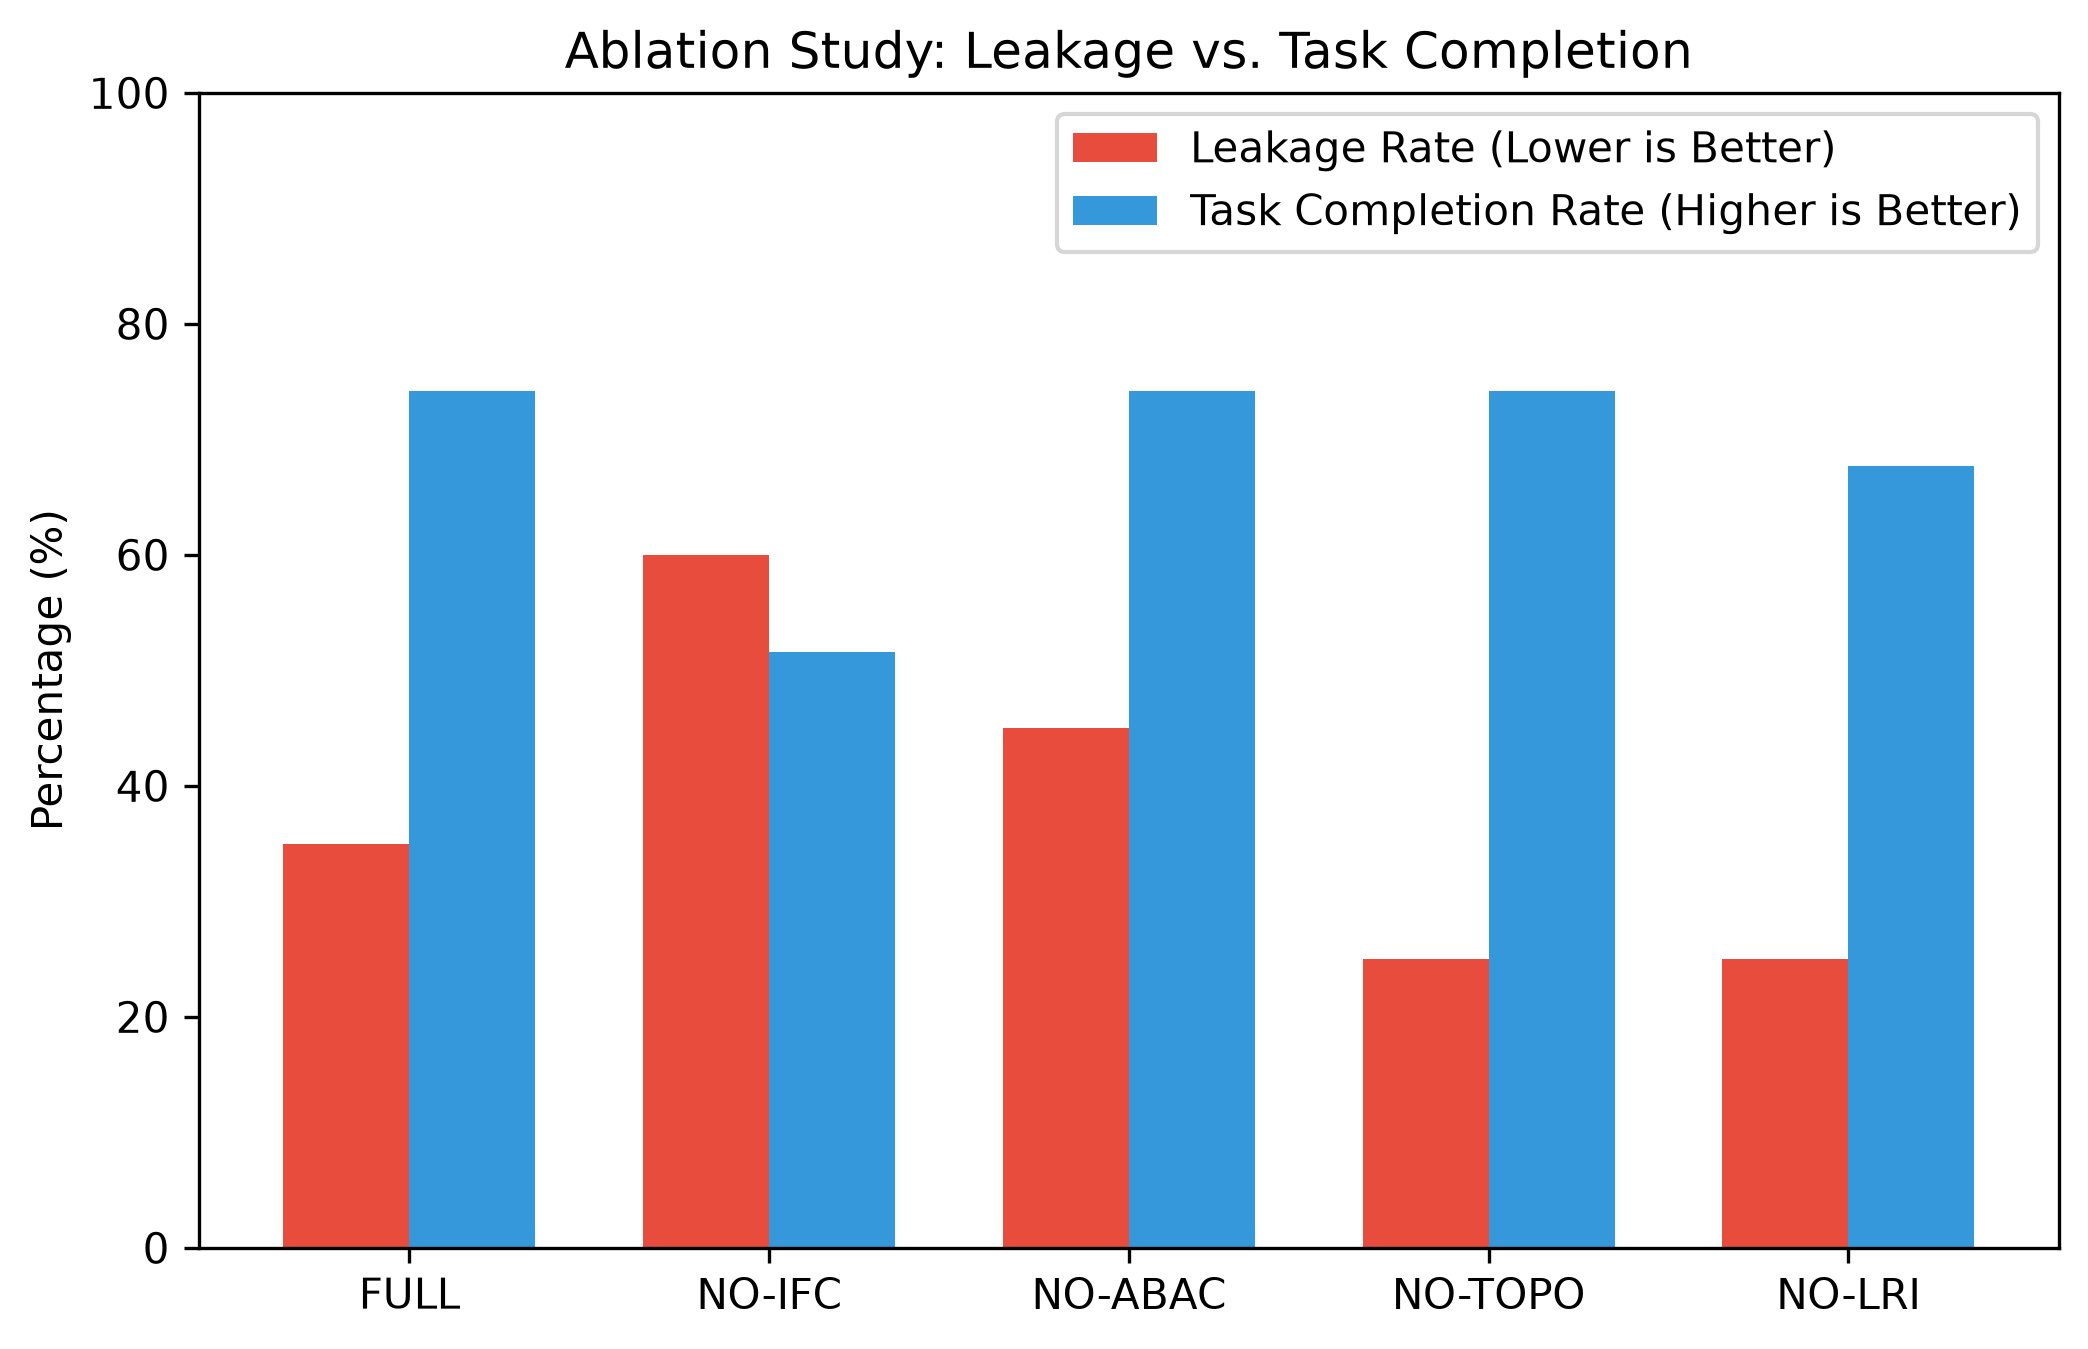
\includegraphics[width=\columnwidth]{ablation_chart.png}
\caption{Empirical trade-off across ablation configurations. Omitting Information Flow Control (NO-IFC) spikes leakage to 60.0\%, while destructive masking reduces downstream LLM task completion to 51.6\%.}
\label{fig:ablation_chart}
\end{figure}

\begin{figure}[htbp]
\centering
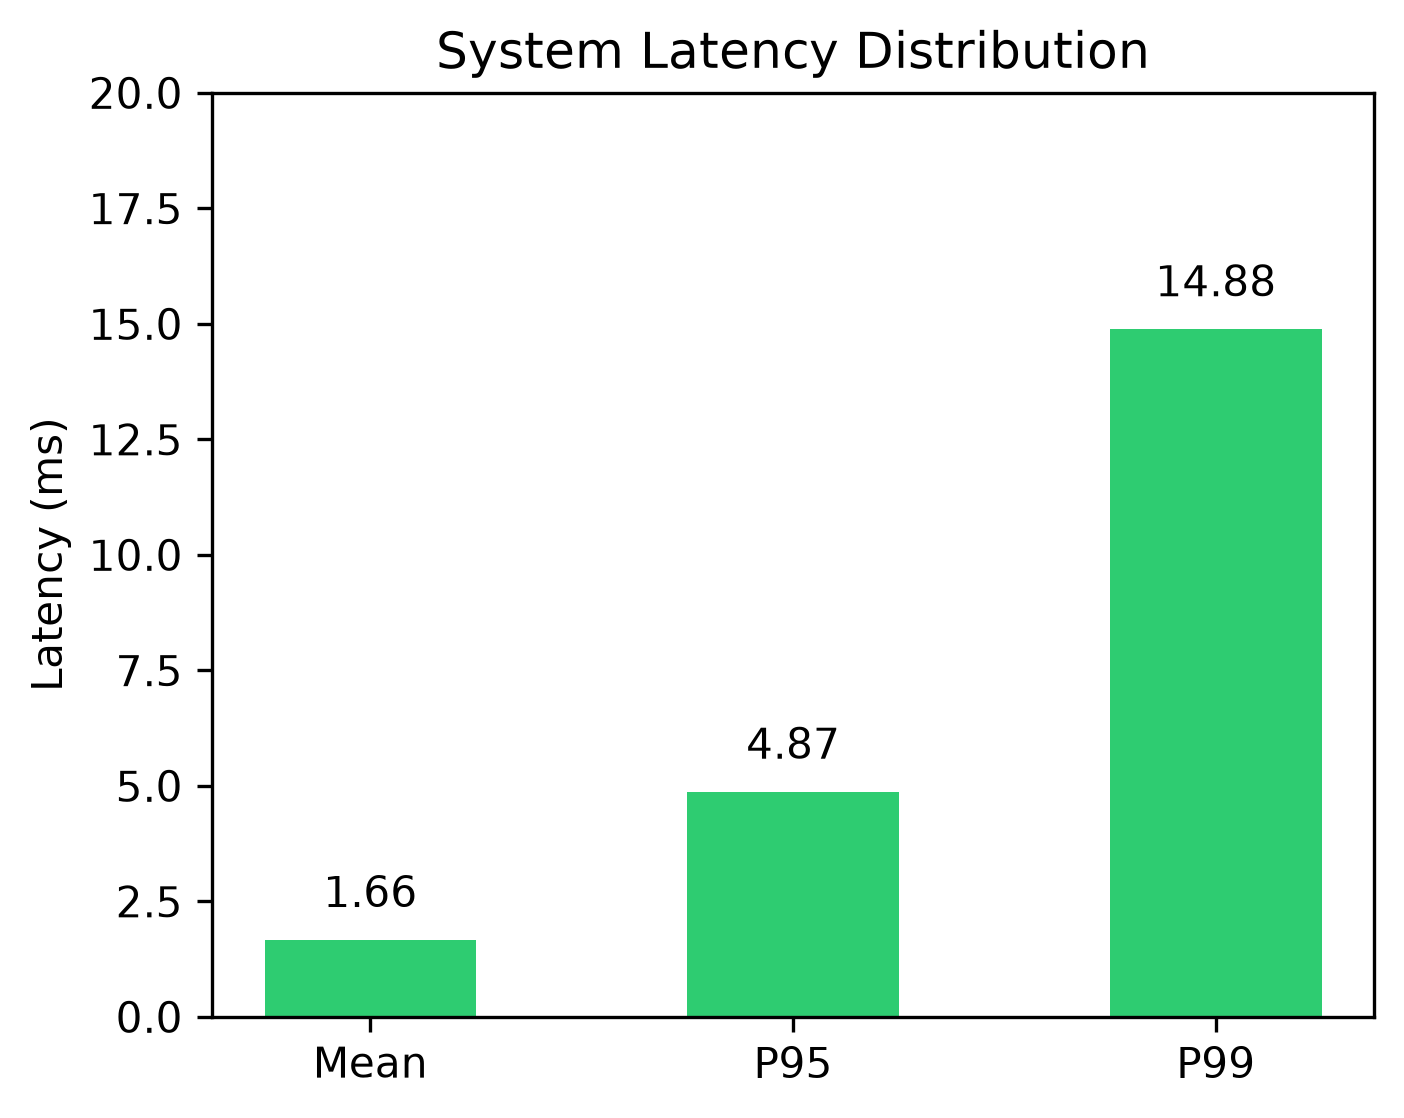
\includegraphics[width=0.85\columnwidth]{latency_chart.png}
\caption{Inline proxy processing latency distribution. Over 95\% of mediation decisions execute in under 4.87\,ms, demonstrating sub-millisecond overhead.}
\label{fig:latency_chart}
\end{figure}

\section{Discussion}
Runtime security mediation in multi-agent workflows introduces an inherent trade-off between privacy enforcement and task performance. Intercepting communication at intermediate agent interfaces mitigates internal channel exposure that bypasses boundary moderation models.

While AgentFlow demonstrates the utility of flow-centric invariant tracking \cite{3}, its reliance on SMT constraint solvers introduces computational overhead that may constrain low-latency agent coordination. PrivAgentShield approaches this challenge by formalizing a quantitative risk index ($LRI^*$) evaluated inline via absorbing Markov chains.

Furthermore, our focus on session-consistent pseudonymization addresses the utility degradation common in naive redaction tools. Downstream agents frequently experience reasoning failures when encountering masked tokens (e.g., *** or [REDACTED]), whereas typed surrogate identifiers allow agents to preserve entity coreference throughout multi-step reasoning processes.

\section{Limitations and Threats to Validity}
\subsection{Limitations}
\begin{enumerate}
    \item \textbf{Detector Quality Dependence:} PrivAgentShield relies on the underlying accuracy of its entity detection engines (Hyperscan, GLiNER, Presidio). Unrecognized entity classes or novel credential formats can lead to understated taint values ($T^*_m$).
    \item \textbf{Obfuscation and Encoding Attacks:} Adversarial agents employing Base64 encoding, cipher routines, or semantic obfuscation may evade regular expression and lightweight NER detectors, requiring deeper transformer probe inspection.
    \item \textbf{Graph Reconstruction Overhead:} In systems characterized by non-deterministic agent generation, dynamically recomputing fundamental matrix $N = (I - Q)^{-1}$ introduces minor computational overhead.
    \item \textbf{Markov Transition Assumptions:} Modeling execution reachability via absorbing Markov chains assumes agent routing probabilities can be estimated from system traces, which may vary under dynamic operational conditions.
    \item \textbf{Reasoning Distortion:} While pseudonymization preserves syntax better than destructive masking, replacement tokens may subtly influence LLM reasoning in domain-specific tasks.
\end{enumerate}

\subsection{Threats to Validity}
\begin{itemize}
    \item \textbf{Internal Validity:} Commercial LLM non-determinism could introduce variance in multi-turn traces across benchmark runs. Experiments must fix sampling temperatures and report confidence intervals across multiple iterations.
    \item \textbf{External Validity:} Synthetic benchmark traces from AgentLeak and AgentDojo may not fully mirror complex enterprise deployments with bespoke internal protocols.
    \item \textbf{Construct Validity:} Operationalizing privacy risk through $LRI^*$ assumes that message taint, clearance dominance, and sink reachability adequately capture information leakage risk.
    \item \textbf{Performance Validity:} Latency measurements must reflect end-to-end multi-agent execution overhead across distributed networks, rather than isolated microbenchmarks.
\end{itemize}

\balance
\section{Conclusion and Future Work}
This paper presented the design and formalization of PrivAgentShield, a policy-aware runtime mediation framework for mitigating sensitive data leakage in multi-agent LLM systems. By formalizing the non-compensatory Leakage Risk Index ($LRI^*$), PrivAgentShield unifies payload sensitivity, lattice clearance dominance, and execution graph reachability into an actionable runtime metric. Enforced through a cascaded three-tier inspection proxy utilizing session-consistent pseudonymization, the architecture provides a systematic path toward securing internal agent coordination channels without requiring foundation model retraining.

Future work will focus on extending PrivAgentShield into a \textbf{Federated Edge AI} architecture, enabling decentralized, privacy-preserving mediation across distributed edge nodes and on-device multi-agent networks. Additional avenues include integrating hardware-accelerated Trusted Execution Environments (TEEs) and formal verification for dynamically evolving agent topologies.

\section*{Data and Code Availability}
The PrivAgentShield source code, empirical evaluation traces, and interactive demonstration dashboard are publicly accessible at \url{https://github.com/Charan359/PrivAgentShield} and hosted live at \url{https://priv-agent-shield-bice.vercel.app/}.

\begin{thebibliography}{00}
\bibitem{1} F. El Yagoubi, G. Badu-Marfo, and R. Al Mallah, ``AgentLeak: A benchmark for internal-channel privacy leakage in multi-agent LLM systems,'' \emph{arXiv preprint arXiv:2602.11510}, 2026.
\bibitem{2} E. Debenedetti et al., ``AgentDojo: A dynamic environment to evaluate attacks and defenses for LLM agents,'' in \emph{Proc. Adv. Neural Inf. Process. Syst. (NeurIPS)}, 2024.
\bibitem{3} A. Standard et al., ``AgentFlow: A flow-centric policy language and framework for securing LLM agent systems,'' \emph{arXiv preprint arXiv:2608.22868}, 2026.
\bibitem{4} S. Geng and H. Chang, ``Contextual integrity and summary collapse in multi-agent LLM handoffs,'' \emph{arXiv preprint arXiv:2608.29028}, 2026.
\bibitem{5} Y. Song et al., ``LeakAgent: RL-based red-teaming for LLM privacy leakage,'' \emph{arXiv preprint arXiv:2602.13840}, 2026.
\bibitem{6} J. Mireshghallah et al., ``Preserving contextual privacy in multi-agent reasoning topologies,'' \emph{arXiv preprint arXiv:2508.07667}, 2025.
\bibitem{7} K. Greshake, S. Abdelnabi, S. Mishra, C. Endres, T. Holz, and M. Fritz, ``Not what you've signed up for: Compromising real-world LLM applications with indirect prompt injection,'' in \emph{Proc. ACM Workshop Artif. Intell. Secur. (AISec)}, 2023, pp. 79--90.
\bibitem{8} L. Zhang et al., ``LLMbda: Dynamic information flow control for language model execution in untyped lambda calculi,'' in \emph{Proc. ACM Program. Lang. (POPL)}, 2025.
\bibitem{9} M. Goyal et al., ``AgentRisk: Quantitative risk scoring and continuous compliance for autonomous LLM agents,'' \emph{IEEE Trans. Dependable Secure Comput.}, 2025.
\bibitem{10} D. E. Denning, ``A lattice model of secure information flow,'' \emph{Commun. ACM}, vol. 19, no. 5, pp. 236--243, 1976.
\bibitem{11} D. E. Bell and L. J. LaPadula, ``Secure computer systems: Mathematical foundations,'' MITRE Corp., Bedford, MA, Tech. Rep. TR-2547, 1973.
\bibitem{12} K. J. Biba, ``Integrity considerations for secure computer systems,'' MITRE Corp., Bedford, MA, Tech. Rep. ESD-TR-76-372, 1977.
\bibitem{13} A. Sabelfeld and A. C. Myers, ``Language-based information-flow security,'' \emph{IEEE J. Sel. Areas Commun.}, vol. 21, no. 1, pp. 5--19, 2003.
\bibitem{14} J. G. Kemeny and J. L. Snell, \emph{Finite Markov Chains}. New York, NY: Springer-Verlag, 1976.
\bibitem{15} H. Inan et al., ``Llama Guard: LLM-based input-output safeguard for human-AI conversations,'' Meta AI Research, Tech. Rep., 2024.
\bibitem{16} Meta AI, ``Llama Guard 3: Specialized safeguards for vision and multimodal deployments,'' Meta AI, Tech. Rep., 2024.
\bibitem{17} T. Rebedea et al., ``NeMo Guardrails: A system for controllable and safe LLM applications,'' in \emph{Proc. Conf. Empirical Methods Nat. Lang. Process. (EMNLP) Syst. Demonstrations}, 2023, pp. 431--445.
\bibitem{18} Microsoft, ``Presidio analyzer and anonymizer for scalable PII detection,'' Microsoft Open Source, 2024.
\bibitem{19} U. Zaratiana, N. Tomeh, P. Holat, and T. Charnois, ``GLiNER: Generalist model for named entity recognition using bidirectional transformers,'' in \emph{Proc. Conf. N. Am. Chapter Assoc. Comput. Linguistics (NAACL)}, 2024.
\bibitem{20} X. Wang et al., ``Hyperscan: A high-performance multiple regex matching engine,'' in \emph{Proc. USENIX Conf. Netw. Syst. Des. Implementation (NSDI)}, 2019, pp. 841--856.
\bibitem{21} LangChain, ``LangGraph: Building stateful multi-agent applications with directed acyclic graphs,'' Tech. Rep., 2024.
\bibitem{22} J. Moura, ``CrewAI: Collaborative multi-agent role-playing architecture,'' Tech. Documentation, 2024.
\bibitem{23} S. Hong et al., ``MetaGPT: Meta programming for a multi-agent collaborative framework,'' in \emph{Proc. Int. Conf. Learn. Representations (ICLR)}, 2024.
\end{thebibliography}

\end{document}
